\begin{table}[H]\centering\small
\begin{tabular}{lrrrrr}
\toprule Round & Dev & Generations & Output tokens & Seconds & Cap rate \\
\midrule
R0 & 26\% & 100 & 24,488 & 56.3 & 70.0\% \\
R1 & 40\% & 100 & 17,510 & 66.5 & 29.0\% \\
R2 & 48\% & 100 & 15,098 & 61.6 & 16.0\% \\
R3 & 36\% & 100 & 14,994 & 52.3 & 14.0\% \\
R4 & 53\% & 394 & 65,839 & 208.5 & 23.4\% \\
\bottomrule\end{tabular}
\caption{Results on 100 dev questions with a 256-token limit per response. Cap rate is the fraction of responses reaching the limit; time covers inference.}
\end{table}
The selected \textbf{fixed-five} configuration scored 56\% dev and \textbf{43\% test} (43/100), with a dev-minus-test gap of 13.0 percentage points. Test evaluation used 500 generations, 86,713 output tokens, and 272.0 seconds.
\begin{figure}[H]\centering
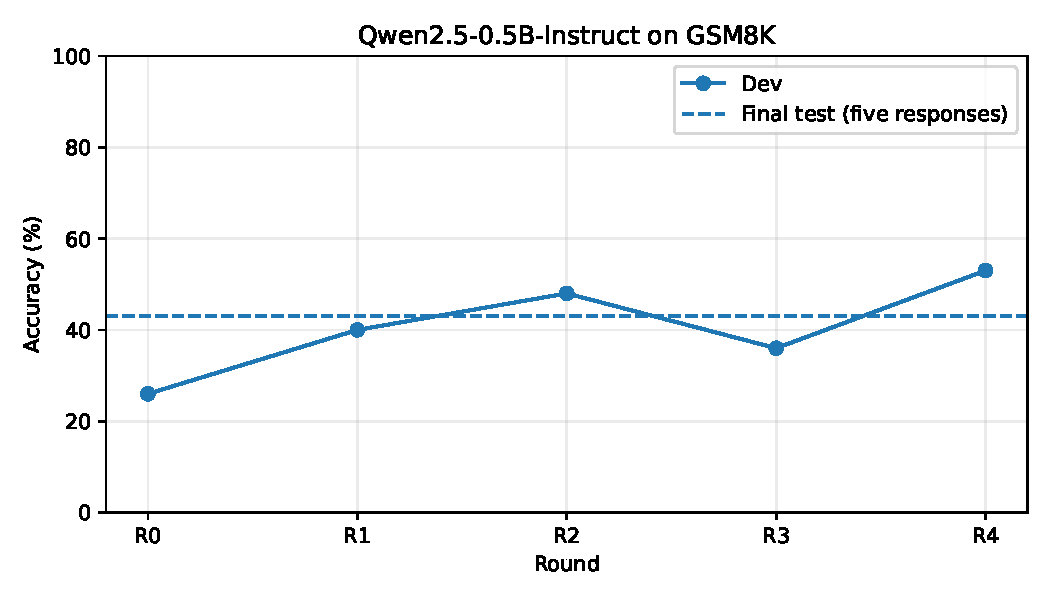
\includegraphics[width=.72\linewidth]{rsi_curve.pdf}
\caption{Dev accuracy across rounds. The dashed line marks the test score of the final five-response configuration. R4 uses the R2 prompt.}
\end{figure}